% TODO varphi??
% TODO curly brace before system?
% TODO proper d
\documentclass{nsart_eng}
\usepackage{cite}
\usepackage{amsmath,amssymb}

% \usepackage{pscyr}
\usepackage[utf8]{inputenc}

\usepackage[russian]{babel}
\usepackage{graphicx}

\year{2016} \volume{0} \nomer{0} \firstpage{1}

\let\le\leqslant
\let\leq\leqslant
\let\ge\geqslant
\let\geq\geqslant


\usepackage{systeme}
\newcommand{\hilb}[1]{\mathcal{H}_{#1}}
\newcommand{\cconj}[1]{\overline{#1}}
\newcommand{\hank}[1]{H_{#1}^{(1)}}

\newcommand{\mcF}{\mathcal{F}}
\newcommand{\mcH}{\mathcal{H}} % ???
\newcommand{\mcI}{\mathcal{I}}
\newcommand{\mcL}{\mathcal{L}} % L2 space
\newcommand{\mcO}{\mathcal{O}} % Big O
\newcommand{\mcP}{\mathcal{P}}


\newcommand{\bbC}{\mathbb{C}} % complex plane
\newcommand{\bbD}{\mathbb{D}} % complex unit disk
\newcommand{\bbH}{\mathbb{H}} % complex upper half-plane TODO add to template
\newcommand{\bbN}{\mathbb{N}}
\newcommand{\bbK}{\mathbb{K}}
\newcommand{\bbR}{\mathbb{R}}
\newcommand{\bbT}{\mathbb{T}} % complex unit circle
\newcommand{\bbZ}{\mathbb{Z}}

\newcommand{\eqdef}{\overset{\mathrm{def}}{=\joinrel=}}

\DeclareMathOperator{\dom}{dom}
\DeclareMathOperator{\ran}{Ran}
\DeclareMathOperator{\rng}{rng}

\newcommand{\todo}[1]{\textcolor{red}{{\large TODO: #1}}}

\newenvironment{elist}{\begin{easylist}[enumerate]}{\end{easylist}}
\newenvironment{ilist}{\begin{easylist}[itemize]}{\end{easylist}}

\newcommand{\myspecial}[1]{\mathrm{#1}}

% imaginary unit
\newcommand{\iu}{{i\mkern1mu}}


\newcommand{\ipcdot}{\ip{\cdot}{\cdot}}
\newcommand{\iip}[2]{[#1,#2]}
\newcommand{\iipcdot}{\iip{\cdot}{\cdot}}

\newcommand{\dsum}{\oplus}
\newcommand{\ddiff}{\ominus}
% indefinite direct sum
\newcommand{\idsum}{[+]}
\newcommand{\iddiff}{[-]}

\DeclarePairedDelimiter{\Vector}{\lparen}{\rparen}

\newcommand{\tit}{\textit}
\newcommand{\cls}{\overline}
\newcommand{\eps}{\varepsilon}


\newcommand{\argmin}{\operatornamewithlimits{argmin}}
\newcommand{\argmax}{\operatornamewithlimits{argmax}}

\renewcommand{\Re}{\operatorname{Re}}
\renewcommand{\Im}{\operatorname{Im}}
\renewcommand{\phi}{\varphi} % TODO is there a prettier way to do that

\newcommand{\eexp}[1]{e^{#1}}

\DeclareMathOperator\atanh{atanh}

% ???
% \newcommand{\abs}[1]{\left| #1 \right|}
% \newcommand{\norm}[1]{\left\lVert #1 \right\rVert}
\newcommand*\Eval[3]{\left.#1\right\rvert_{#2}^{#3}}
\usepackage{mathtools} % xmapsto, \Vector

\DeclarePairedDelimiter{\abs}{\lvert}{\rvert}
\newcommand{\eexp}[1]{e^{#1}}
\newcommand{\iu}{{i\mkern1mu}}
\renewcommand{\Re}{\operatorname{Re}}
\renewcommand{\Im}{\operatorname{Im}}

\begin{document}

% TODO ??
\title[короткое название статьи]
{НАЗВАНИЕ СТАТЬИ}

\author[Д.\,А.~Герасимов]
{$^1$Д.\,А.~Герасимов}

\address{
$^1$ Санкт-Петербургский Национальный Исследовательский Университет Информационных Технологий, \\
Механики и Оптики,\\
Кронверкский пр., 49, Санкт-Петербург, 197101, Россия}

\email{karlicoss@gmail.com}

УДК ???.??, ???.???.?% insert UDK

\begin{abstract}
Рассматривается задача рассеивания на квантовом графе $\Gamma$, представляющем из себя кольцо $\Omega$, связянное с волноводом $\delta$-граничным условием (TODO как оно нормально называется???), параметризованным вещественной константой $a$. Изучается поведение системы при различных $a$, и полнота резонансных состояний оператора Шредингера графа $\Gamma$ в пространстве $\mcL_2(\Omega)$.
\end{abstract}

\keywords{задача рассеяния, квантовый граф, резонансы, уравнение Шредингера}

\maketitle

\section{Введение}

Квантовый граф — широко используемая модель наносистемы \cite{1, 2, 3, 4}. Если граф $\Gamma$ состоит только из конечного числа ребер конечной длины, его гамильтониан имеет чисто дискретный спектр, и его собственные функции образуют полную систему в $\mcL_2(\Gamma)$. Если же граф $\Gamma$ представляет из себя резонатор $\Omega$ с полубесконечными ребрами, в спектре будет присутствовать непрерывная часть и резонансы, индуцированные собственными числами гамильтониана резонатора $\mcH_\Omega$. Резонансные состояния оператора Шредингера не принадлежат пространству $\mcL_2(\Gamma)$, однако, при сужении их на конечный домен $\Omega$, становятся квадратично интегрируемыми и лежат в пространстве $\mcL_2(\Omega)$. Для многих приложений (TODO каких? ссылки?) интересно знать, формируют ли полную систему резонанстные состояния графа $\Gamma$ в пространстве $\mcL_2(\Omega)$ резонатора.

\section{Цель работы и постановка задачи}
В статье TODO ссылка была показана полнота резонансных функций на графе с резонатором, состоящим из отрезка с $\delta$-граничным условием. Естественным предположением является что произвольный резонатор состоящий из конечного числа ребер конечной длины должен обладать похожими свойствами, однако, это не так. В этой работе исследуется резонатор, состоящий из кольца и показывается неполнота резонансных состояний на этом кольце.

\section{Терминология и вспомогательные сведения}
В общем виде волновые функции, являющиеся решениями уравнения Шредингера слева и справа от резонатора имеют вид:
\[
\psi_L(x) = A \eexp{\iu k x} + B \eexp{-\iu k x}
\]
\[
\psi_R(x) = C \eexp{\iu k x} + D \eexp{-\iu k x}
\]

S-матрица (матрица рассеяния) выражает зависимость исходящей волны от входящей:
\[
\begin{pmatrix} B \\ C \end{pmatrix} = S \begin{pmatrix} A \\ D \end{pmatrix}
\]

Для скалярных внутренних функций $\phi$ существует критерий отстутствия сингулярного множителя \cite[стр. 99]{nikolskii}:
\[
\lim\limits_{r = 1} \int\limits_{\bbT} \log \abs{\phi(r \zeta)} d m(\zeta) = 0
\]

Так как $\det S$ является скалярной внутренней функцией, мы можем воспользоваться данным критерием для исследования полноты системы резонантных состояний.
% $\det S$ — произведение Бляшке-Потапова $\iff$ TODO ??? 

\section{Модель исследования}
\begin{figure}[!htb]
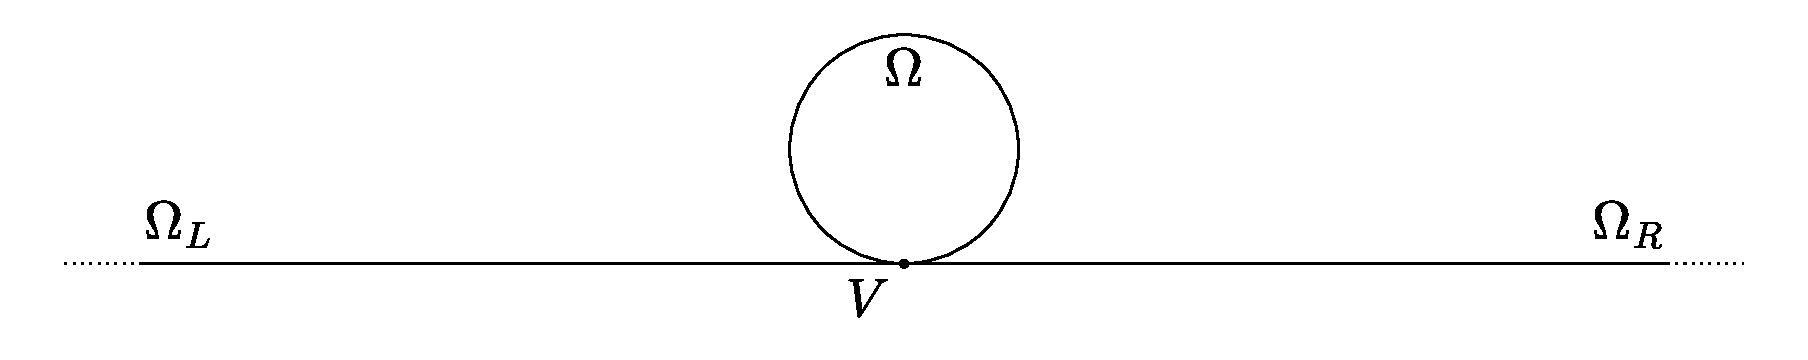
\includegraphics[width=\textwidth,keepaspectratio]{graph.eps}
\caption{квантовый граф $\Gamma$, состоящий из полубесконечных ребер $\Omega_L, \Omega_R$ и рассеивателя $\Omega$, представляющего из себя окружность длиной $1$.}
\end{figure}

Мы рассматриваем случай рассеяния волны c волновым вектором $k$, приходящей слева направо. Таким образом, волновые функции на различных частях графа принимают следующий вид:

\begin{align*}
\psi_L(x) &= \eexp{\iu k x} + R \eexp{-\iu k x} \\
\psi_R(x) &= T \eexp{\iu k x}\\
\psi_\Omega(x) &= P \sin(k x) + Q \cos(k x)
\end{align*}
, где $R$ и $T$ — коэффициенты отражения и прохождения волны. Так как система симметрична, ее матрица рассеяния принимает вид
$S(k) = \begin{pmatrix} R(k) & T(k) \\ T(k) & R(k) \end{pmatrix}$.

В вершине $V$ мы ставим граничное условие Дирихле на волновую функцию, и $\delta$-условие со связью $a$ на ее производную:

\begin{align*}
\psi_L(0) = \psi_R(0) = \psi_\Omega(0) = \psi_\Omega(1) \\ 
-\psi'_L(0) + \psi'_\Omega(0) - \psi'_\Omega(1) + \psi'_R(0) = a \psi_L(0)
\end{align*}


\section{Вычисление S-матрицы}
Определим коэффициенты прохождения и отражения, решив систему линейных уравнений:
\begin{align*}
& 1 + R &= T \\
& 1 + R &= Q \\
& Q \cos k + P \sin k &= T \\
& -P k \cos k + Q k \sin k + P k + \iu R k + \iu T k - \iu k &= T a
\end{align*}

Решив систему, получаем:

\begin{align*}
R(k) = -\frac{2 \, k \cos\left(k\right) + a \sin\left(k\right) - 2 \, k}{2 \, k \cos\left(k\right) + {\left(a - 2 i \, k\right)} \sin\left(k\right) - 2 \, k} \\
T(k) = -\frac{2 i \, k \sin\left(k\right)}{2 \, k \cos\left(k\right) + {\left(a - 2 i \, k\right)} \sin\left(k\right) - 2 \, k}
\end{align*}
, подставляя полученные значения коэффициента прохождения и отражения в S-матрицу, получаем:
\[
\det S = 
\frac
{\cos\left(k\right) + {\left(\frac{a}{2 k} + i\right)} \sin\left(k\right) - 1}
{\cos\left(k\right) + {\left(\frac{a}{2 k} - i\right)} \sin\left(k\right) - 1}
\]


\section{Исследование полноты при $a=0$}
Рассмотрим случай $a=0$:
\[
\det S
= \frac
{\cos\left(k\right) + \iu \sin\left(k\right) - 1}
{\cos\left(k\right) - \iu \sin\left(k\right) - 1}
= \frac{\eexp{\iu k} - 1}{\eexp{-\iu k} - 1}
= -\eexp{i k}
\]

\[
\ln \abs{\det S} = \ln \eexp{- \Im k} = -\Im k
\]

% Преобразование Кэли: $\zeta = \frac{k - i}{k + i}$, обратное: $k = \iu \frac{1 + \zeta}{1 - \zeta}$.

Вычислим интеграл в пространстве единичного диска, для этого применим обратное преобразование Кэли $k \to \iu \frac{1 + \zeta}{1 - \zeta}$ к подынтегральной функции: $\Im k \to \Im \left( \iu \frac{1 + \zeta}{1 - \zeta} \right) $.

\[
  \lim\limits_{R = 1} \int\limits_{\abs{\zeta} = R} \ln \abs{\det S(\zeta)} d \zeta
= \lim\limits_{R = 1} \int\limits_{\abs{\zeta} = R} \Im \left( \iu \frac{1 + \zeta}{1 - \zeta} \right)  d\zeta = \dots
\]

Перейдем в полярные координаты: $\zeta \to R \eexp{\iu \phi}, d\zeta \to R \iu \eexp{\iu \phi}$:
\[
\dots = \lim\limits_{R = 1} \int\limits_{\abs{\zeta} = R} \Im \left( \iu \frac{1 + R \eexp{\iu \phi}}{1 - R \eexp{\iu \phi}} \right) R \iu \eexp{\iu \phi} d\phi
\]

Комплексный интеграл складывается из сумм интегралов действительной и мнимной части подынтегрального выражения. Рассчитаем мнимую часть:

\begin{align*}
\Im \left(  \Im \left( \iu \frac{1 + R \eexp{\iu \phi}}{1 - R \eexp{\iu \phi}} \right) R \iu \eexp{\iu \phi} \right)
 &= R \Re \left(  \Re \left( \frac{1 + R \eexp{\iu \phi}}{1 - R \eexp{\iu \phi}} \right) \eexp{\iu \phi} \right) \\
 &= R \Re \left( \frac{1 + R \eexp{\iu \phi}}{1 - R \eexp{\iu \phi}} \right) \Re \left(   \eexp{\iu \phi} \right) \\
 &= R \Re \left( \frac{(1 + R \eexp{\iu \phi}) (1 - R \eexp{-\iu \phi}) }{(1 - R \eexp{\iu \phi}) (1 - R \eexp{-\iu \phi})} \right) \cos \phi \\
 &= R \Re \left( \frac{1 - R^2 + 2 \iu R \sin \phi}{1 + R^2 - 2 R \cos \phi} \right) \cos \phi \\
 &= R \frac{1 - R^2}{1 + R^2 - 2 R \cos \phi} \cos \phi \\
 % NOTE calculate the integral properly?
 &= 2 \pi R^2
\end{align*}

Можно видеть, что предел мнимой части при $R \to 1$ равен $2 \pi$, следовательно, по критерию полноты, система резонатных состояний графа $\Gamma$ не является полной на кольце $\Omega$.

% Формула с нумерацией:
% \begin{equation} \label{eq1}
% \alpha (t) = \frac{ \beta (t)}{\gamma (t)}.
% \end{equation}

% Многострочные формулы можно задавать так:
% \begin{multline} \label{eq2}
% \sum\limits_{n=0}^\infty  {\frac{{f^{\left( n \right)} \left( {x_0 } \right)}}{{n!}}\left( {x - x_0 } \right)^n }  = \\
% = f\left( {x_0 } \right) + \frac{{f'\left( {x_0 }
% \right)}}{{1!}}\left( {x - x_0 } \right) +
%  \frac{{f''\left( {x_0 } \right)}}{{2!}}\left( {x - x_0 } \right)^2 + \dots +
%  \frac{{f^{\left( n \right)} \left( {x_0 } \right)}}{{n!}}\left( {x - x_0 } \right)^n  + \dots
% \end{multline}

% Ссылки на формулы задаются так  (\ref{eq1}).

% \subsection{Название подпараграфа 2}
% Текст подпараграфа 2.

\section{Заключение}
TODO ????
% Было показано, что полнота резонансных состояний в пространстве резонатора 

% \section*{Благодарности}
% Текст.

\begin{thebibliography}{99}
\bibitem{1} P.Kuchment, \textit{Waves in Random Media}, \textbf{12}(4), R1-R24 (2002)

\bibitem{2} I.S. Lobanov, A.I. Trifanov, E.S. Trifanova, \textit{Nanosystems: Phys. Chem. Math.}, \textbf{3}(4), 512-523 (2013).

\bibitem{3} P.Exter. J.P. Keating, P. Kuchment, T. Sunada, A. Teplyaev (eds.), \textit{Analysis on Graphs and Its Applications}. Proc. Symp. Pure Math., 77 (Providence, RI: Amer. Math. Soc.) (2008)

\bibitem{4} I.Yu. Popov, A.N. Skorydina, I.V. Blinova, \textit{J. Math. Phys.}, \textbf{55}, 033504 (2014)

\bibitem{nikolskii} N.K. Nikol'skii. {\it Treatise on the Shift Operator: Spectral Function Theory}.  Springer Berlin Heidelberg,  491~p. (2012)

% \bibitem{2}
% Автор~В.\,В., Автор~Г.\,Г. Название статьи. {\it Название журнала}, {\bf 1} (5), С 1 -- 3. (2000)

% \bibitem{3}
% Автор~Д.\,Д., Автор~Е.\,Е. Название доклада. Сборник трудов конференции "Конференция", место и дата, С. 47 -- 49

% \bibitem{3}
% Автор~Ж.\,Ж., Автор~З.\,З. Название статьи.  2010.
% URL/arXiv: http://books.ifmo.ru/ntv.

% \bibitem{4}
% Название патента: патент 1111111 Россия MMM H04 B 1/36, Иванов И.И., владелец патента. OGOGO, N 2000131517/09, Bull. N 12, 3 с.

\end{thebibliography}

\end{document}
